\documentclass{article}

% Language setting
% Replace `english' with e.g. `spanish' to change the document language
\usepackage[spanish]{babel}
\usepackage[numbers]{natbib}


% Set page size and margins
% Replace `letterpaper' with `a4paper' for UK/EU standard size
\usepackage[a4paper,top=2cm,bottom=2cm,left=3cm,right=3cm,marginparwidth=1.75cm]{geometry}
\setlength{\parindent}{0pt}


% Useful packages
\usepackage{amsmath}
\usepackage{graphicx}
\usepackage[colorlinks=true, allcolors=blue]{hyperref}
\usepackage{xcolor}
\usepackage{listings}
\usepackage{float}

\lstnewenvironment{Rcode}[1][]{
\lstset{
    language=R,
    basicstyle=\small\ttfamily,
    columns=fullflexible,
    keepspaces=true,
    xleftmargin=1em,
    framexleftmargin=1em,
    #1
    }
}{}



\title{Manual de Usuario de ATLAS}
\author{Maria del Valle Alonso de Caso Ortiz}
%%Empezado el 12 de febrero de 2024

\begin{document}
\maketitle

%\begin{abstract}
%Your abstract.
%\end{abstract}

%%--------------------------------------------------------
%% 1. INTRO
%%--------------------------------------------------------

\section{Introducción a ATLAS.}

ATLAS es una plataforma de análisis de ciencia abierta que se puede instalar localmente dentro de su institución para realizar análisis en una o varias bases de datos observacionales que se han estandarizado al Modelo de Datos Común OMOP V5 y puede facilitar el intercambio de diseños de análisis con cualquier otra organización dentro de la comunidad OHDSI que haya adoptado los mismos estándares y herramientas de ciencia abierta \cite{OHDSIAtlasWiki}


%%---------------------------------------------------------------
%% 2. DESPLIEGUE
%%-------------------------------------------------------------------

\section{Despligue de la herramienta.}

ATLAS puede desplegarse de múltiples maneras, desde formas muy sencillas que no necesitan ninguna instalación local hasta la implementación local más pura y compleja. En este manual de usuario se presentan todas las formas de implementar ATLAS de menor a mayor complejidad: ATLAS demo [\ref{cap:ATLASdemo}], ATLAS Broadsea [\ref{cap:AtlasBroadsea}], ATLAS AWS [\ref{cap:AtlasAWS}] y ATLAS local [\ref{cap:ATLASlocal}]

%%--------------------------------------------------------------
%% 2.1 ATLAS DEMO
%%--------------------------------------------------------------    

\subsection{ATLAS demo} \label{cap:ATLASdemo}

ATLAS demo es una instanciación, disponible públicamente de forma gratuita, que permite acceder a una versión online de la herramienta. Es la forma más fácil de tener un primer contacto con la herramienta, pues solo es necesario acceder a través del  \href{https://atlas-demo.ohdsi.org/}{link} que nos facilita la página web oficial de OHDSI, desde la pestaña \href{https://atlas-demo.ohdsi.org/}{software tools}. \\

\begin{figure}[H]
    \centering
    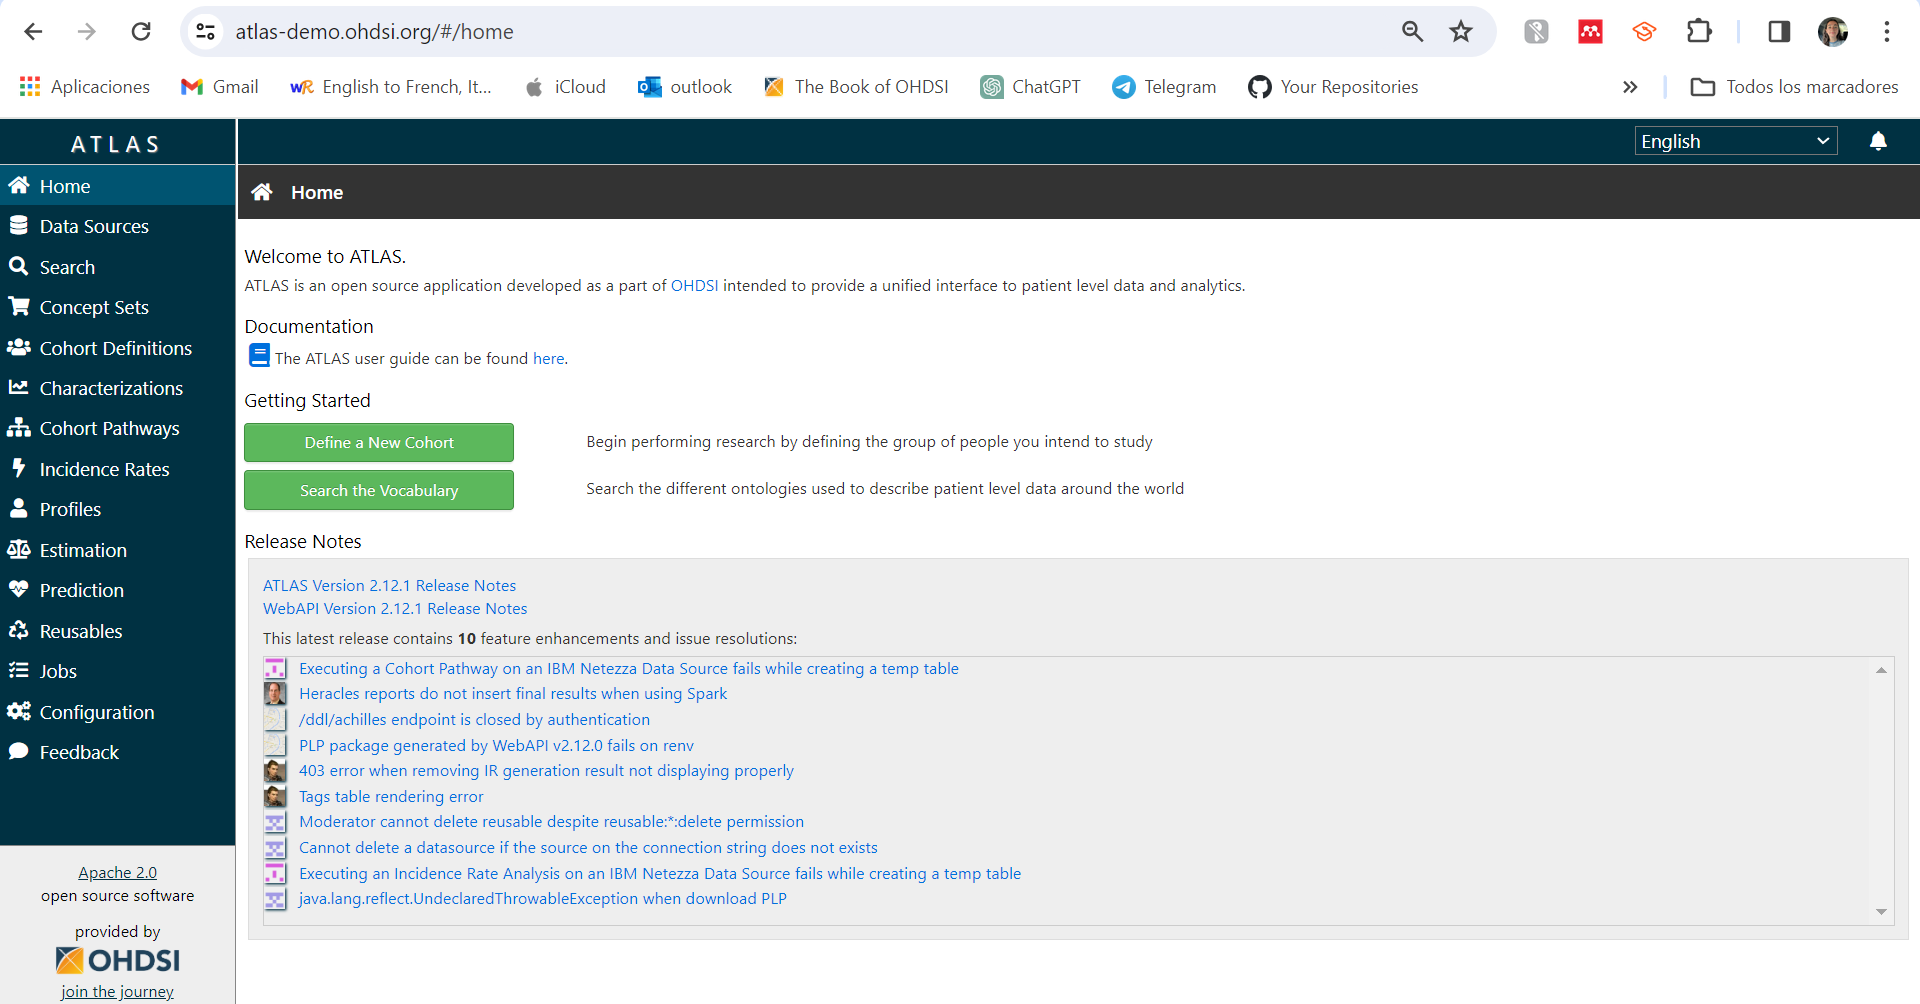
\includegraphics[width=0.90\textwidth]{images/atlasDemo.png}
    \caption{Captura de pantalla de menú principal de ATLAS demo}
\end{figure}

A pesar de ser una demo, no debe subestimarse su potencial de operación. Esta versión online de la herramienta, ofrece soporte para cuatro bases de datos (demo) de OHDSI: ATLASPROD, Common Evidence Model, SYNPUF 1K y SYNPUF 5\%. Además, al ser una herramienta disponible online públicamente para cualquier usuario, almacena la información que deposita cada usuario tras su uso, es decir, almacena gran cantidad de ejemplos de estructuras de cohortes, caracterización... aunque hay que tener en cuenta que al ser estructuras definidas por usuarios no administradores, pueden ser incorrectas. No obstante, no deja de ser un gran repositorio público para empezar a trabajar con ATLAS. \\

\begin{figure}[H]
    \centering
    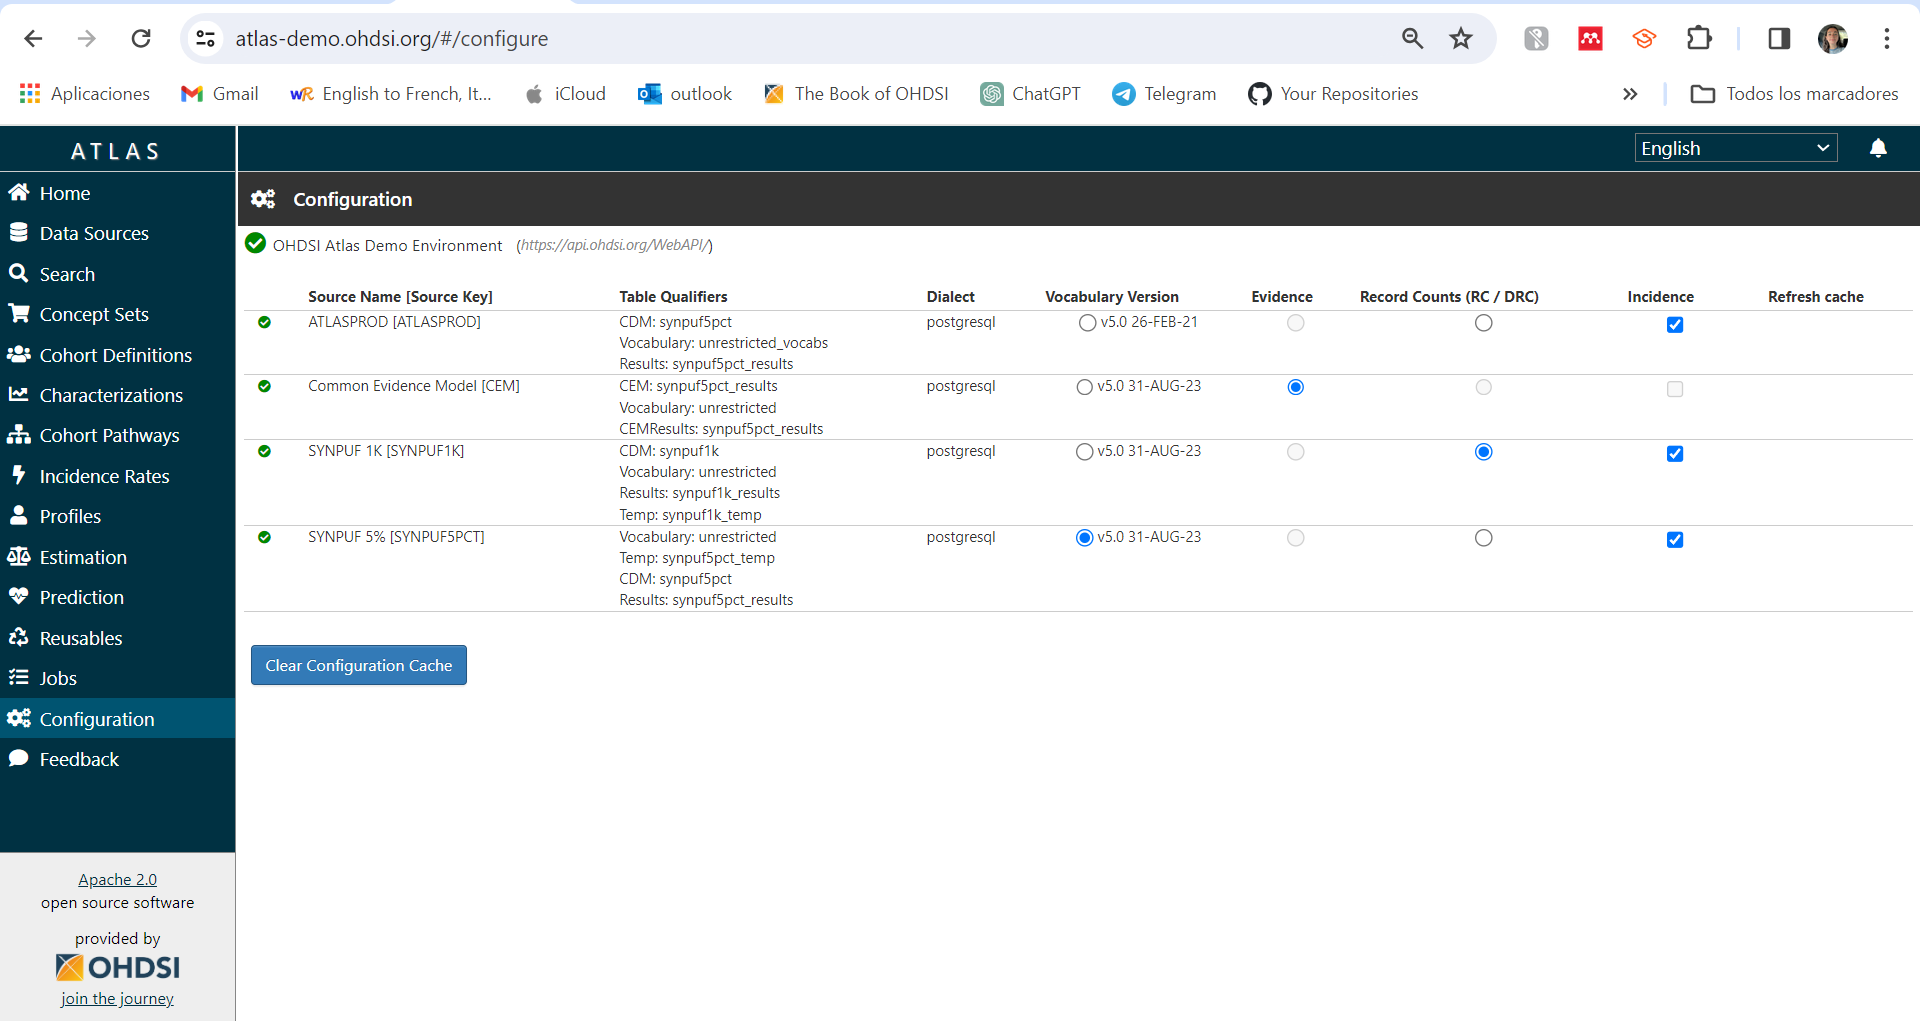
\includegraphics[width=0.90\textwidth]{images/atlasDemo(1).png}
    \caption{Captura de pantalla de bases de datos que utiliza ATLAS demo}
\end{figure}

\begin{figure}[H]
    \centering
    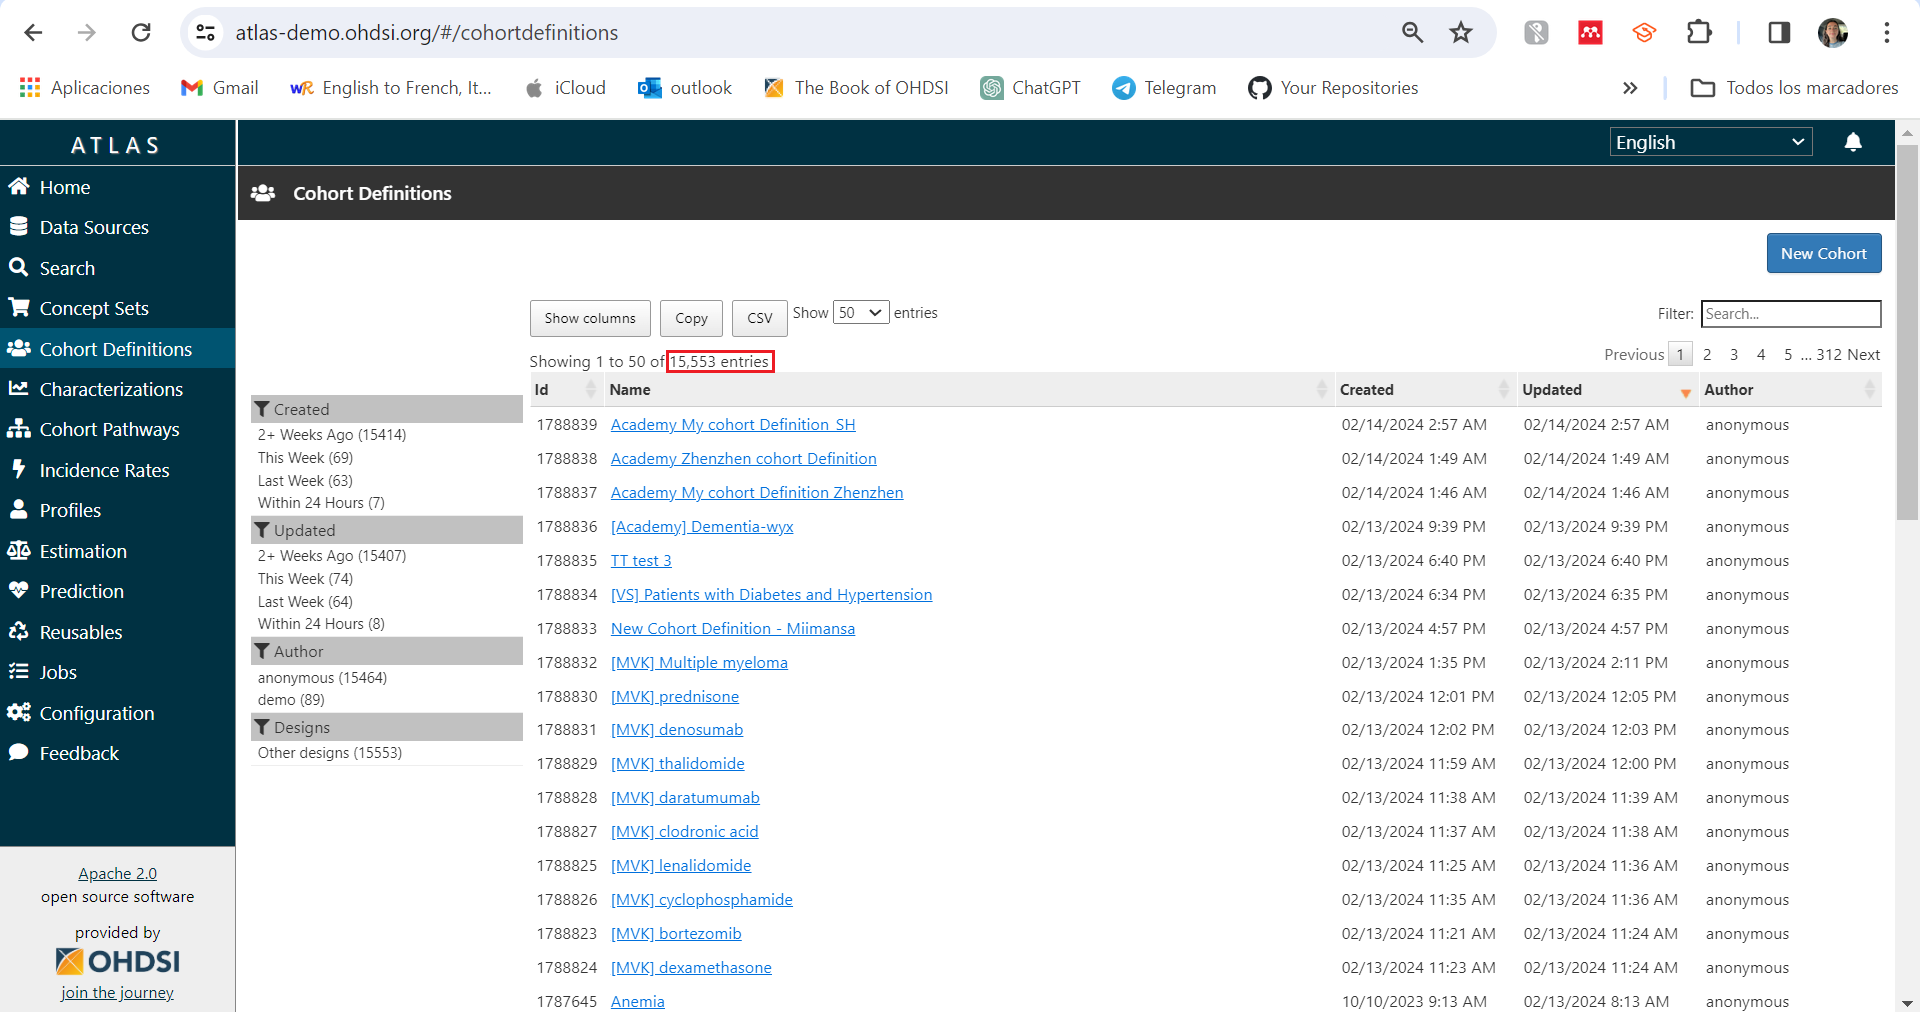
\includegraphics[width=0.90\textwidth]{images/atlasDemo(2).png}
    \caption{Captura de pantalla señalando el número de entradas de definición de cohorte que almacena ATLAS demo}
\end{figure}


Frente a este despliegue online, sin necesidad de descargar ni instalar ningún programa ni software adicional, se encuentra la opción de desplegar la herramienta de manera local, para limpiar la herramienta de todos estos datos de otros usuarios y trabajar localmente con información propia. \\

Sin embargo, esta instalación puede llegar a ser bastante compleja puesto que hay muchos componentes con dependencias que deben ser considerados y configuraciones que deben ser establecidas. Por esta razón, dos iniciativas han desarrollado estrategias integradas de implementación que permiten instalar toda la pila como un paquete, utilizando algunas formas de virtualización: Broadsea \ref{cap:AtlasBroadsea} y Amazon Web Services (AWS) \ref{cap:AtlasAWS}. \cite{TheBookOfOhdsi}

%%----------------------------------------------------------------
%% 2.2 ATLAS Docker
%%--------------------------------------------------------------

\subsection{ATLAS docker - Broadsea}\label{cap:AtlasBroadsea}

Broadsea es un proyecto basado en Docker que permite desplegar de manera consistente aplicaciones web de OHDSI (Atlas, Ares y Hades) junto con las dependencias de base de datos y redes necesarias para ejecutar esas herramientas. Broadsea ha permitido a los investigadores experimentar con herramientas de OHDSI sin necesidad de tener una experiencia técnica significativa o incurrir en gastos elevados. Debido al enfoque basado en Docker, la configuración es consistente, independientemente del sistema operativo o hardware.  \cite{Broadsea3.0}

%-------------------------------------------------------------
\subsubsection{Despliegue de Docker}

El despliegue de ATLAS en Docker es muy sencillo y está bien documentado en el  \href{https://github.com/OHDSI/Broadsea}{repositorio de github} de Broadsea. De hecho, la propia organización considera Broadsea la manera más sencilla de instalar (y actualizar) Docker. Igualmente, en este manual detallaremos nuevamente los pasos para la configuración y despliegue de la herramienta.\\

\textbf{Requisitos para el despliegue}
\begin{enumerate}
    \item Descargar e instalar Docker. Lo más sencillo es seguir las instrucciones de la \href{https://docs.docker.com/engine/install/}{página web oficial} para la descarga y seguir la configuración por defecto para la instalación.
    
    \item Descargar e instalar Git. Lo más sencillo es seguir las instrucciones de la \href{https://git-scm.com/downloads}{página web oficial} para la descarga y seguir la configuración por defecto para la instalación.
\end{enumerate}

\textbf{Deployment}
\begin{enumerate}
    \item El primer paso para desplegar ATLAS es clonar localmente el repositorio de GitHub de Broadsea. Una forma rápida de hacerlo es, desde la terminal, introducir la siguiente línea.

\begin{lstlisting}[language=sh]
        git clone https://github.com/OHDSI/Broadsea.git
\end{lstlisting}

    \item El segundo paso, es desplegar el contenedor docker. Para ello, desde la terminal, nos situamos en la carpeta donde se ha copiado el repositorio de github de Broadsea. Podemos utilizar el comando cd con la ruta al repositorio local.

\begin{lstlisting}[language=sh]
        cd ruta\del\repositorio\Broadsea\local
\end{lstlisting}

    Una vez nos encontramos en la carpeta raíz del repositorio, ejecutamos el siguiente comando, que instalará el contenedor docker en nuestro ordenador.

\begin{lstlisting}[language=sh]
    docker compose pull && docker-compose --profile default up -d
\end{lstlisting}

\end{enumerate}

%---------------------------------------------------------------
\textbf{Comprobación de despliegue correcto} 

Podemos comprobar que se ha instalado correctamente el contenedor de Broadsea en nuestro ordenador de distintas formas, así como comprobar su correcto despliegue y ejecución e instalación de parámetros de configuración. En esta sección vamos a abordar todos estos puntos.

\begin{enumerate} 

    \item La forma más sencilla de interactuar con el contenedor de Broadsea es a través de Docker Desktop. Ejecutando dicho programa, en la sección \textit{"containers"} se muestran todos los contenedores que están corriendo en el equipo. En este caso, debe aparecer un multi-contenedor llamado "broadsea" que contenga seis contenedores, tal y como se muestra en la Figura \ref{fig:dockerDesktop}.
    
    Mediante el panel de control de Docker se puede iniciar, pausar o detener cada contenedor (o todos a la vez) fácilmente y en cualquier momento. Por esto se dice que Broadsea es \textit{a-la-carte}.
    
\begin{figure}[H]
    \centering
    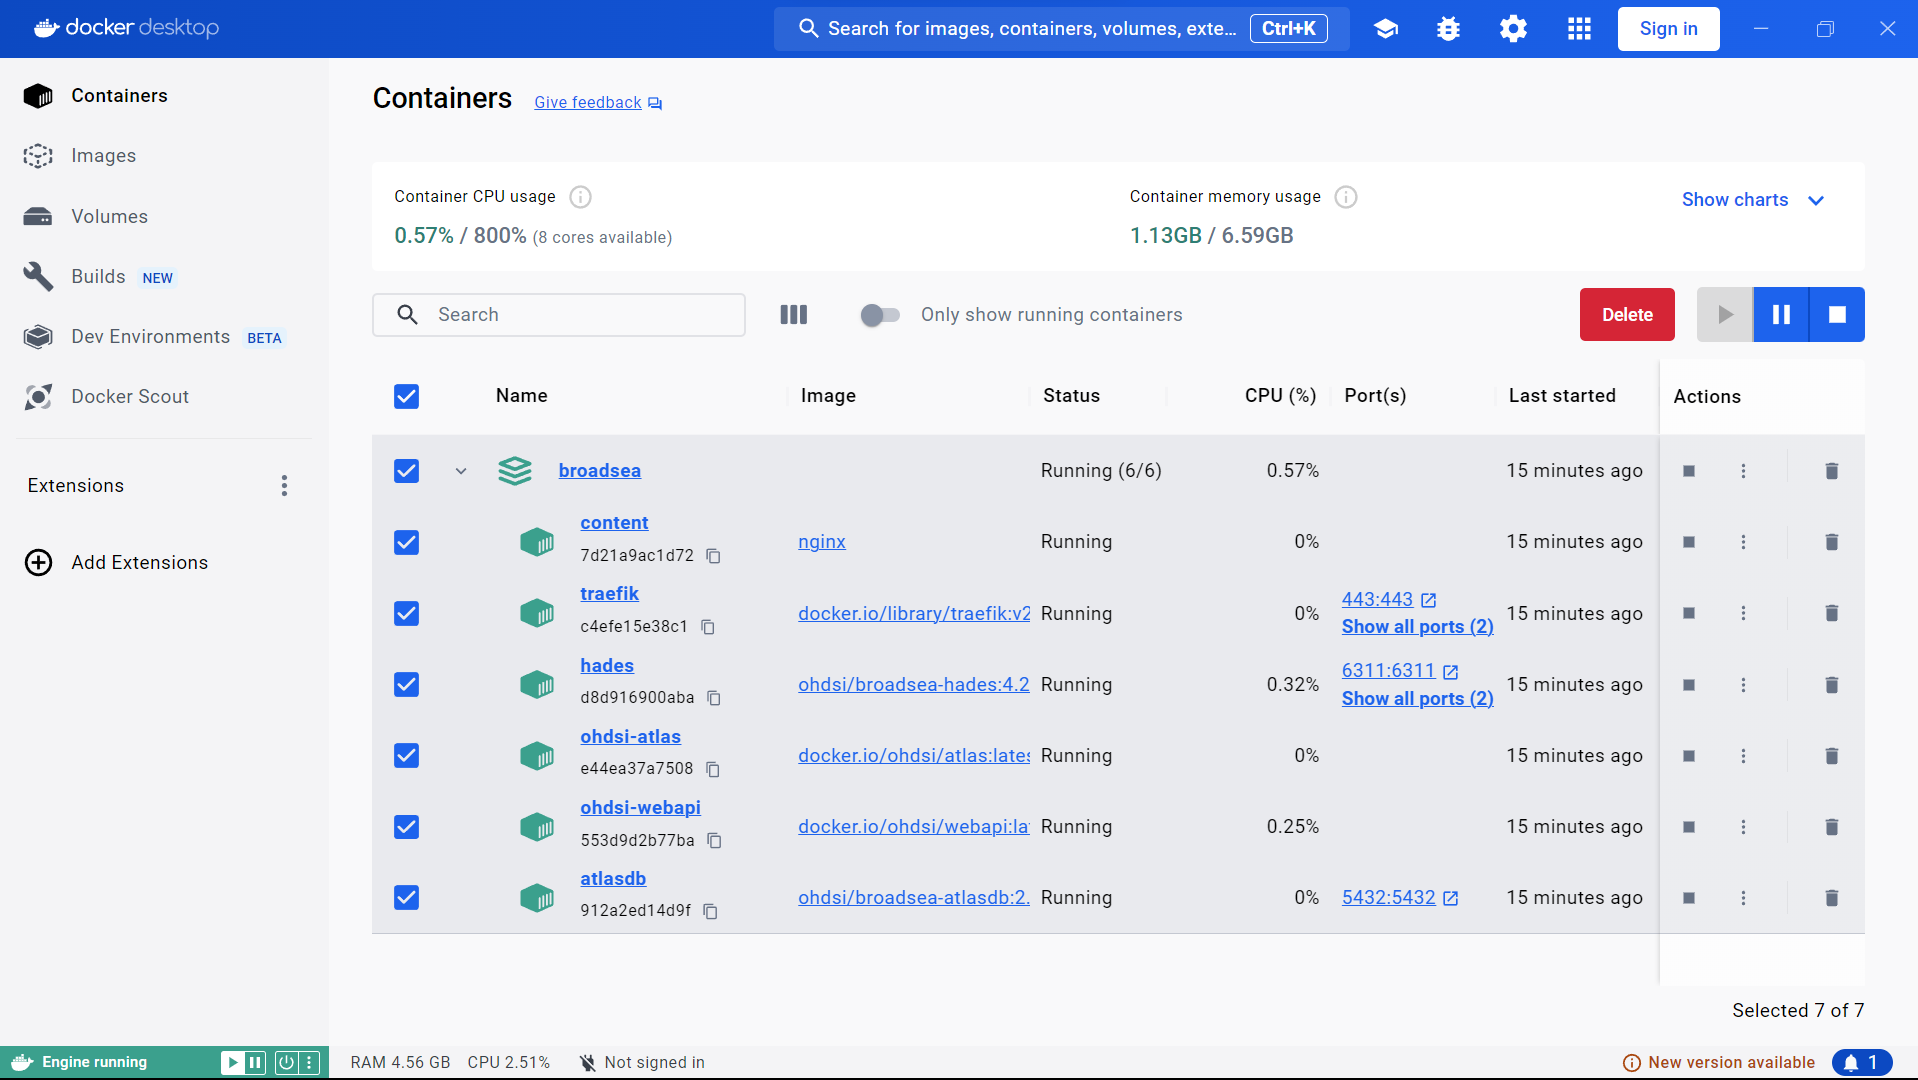
\includegraphics[width=0.90\textwidth]{images/dockerDesktop.png}
    \caption{Captura de pantalla del contenedor Broadsea en Docker Desktop}
    \label{fig:dockerDesktop}
\end{figure}

    \item Otra forma de comprobar que Docker está ejecutando el contenedor correctamente en nuestro dispositivo es mediante la terminal, a través del comando ''docker ps'', que muestra un listado de todos los contenedores que se están ejecutando. De esta forma deberían mostrarse los seis contenedores pertenecientes a broadsea, tal y como se muestra en la Figura \ref{fig:dockerCMD}

\begin{figure}[H]
    \centering
    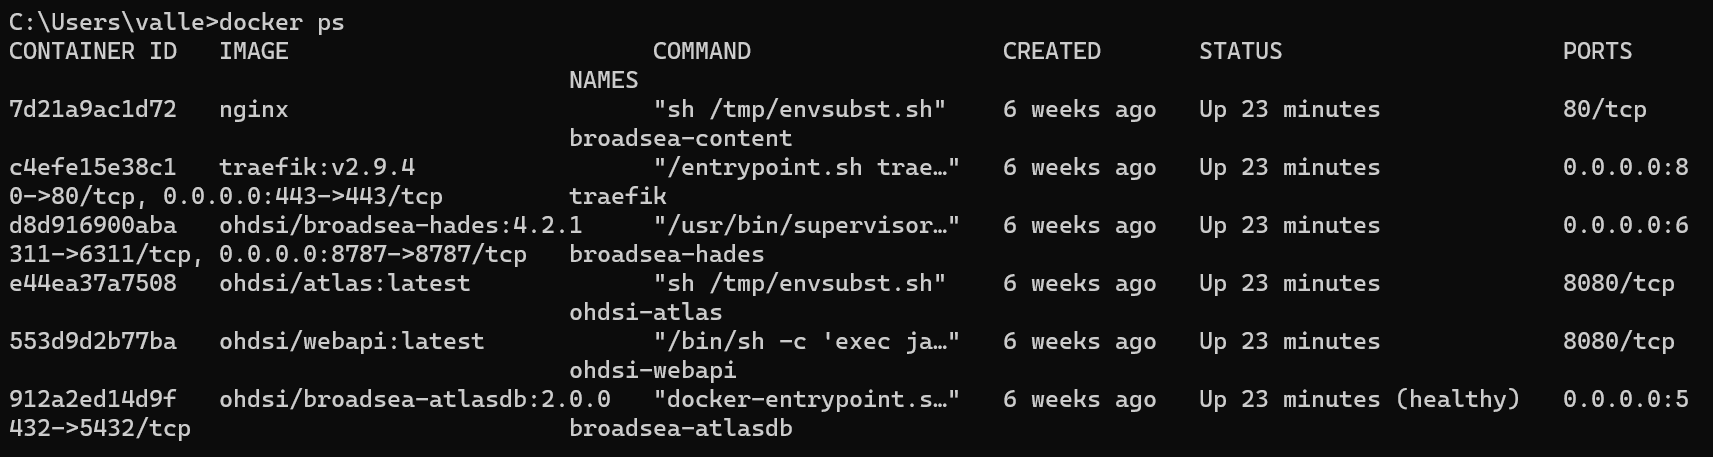
\includegraphics[width=0.90\textwidth]{images/dockerCMD.png}
    \caption{Captura de pantalla del comando ''docker ps'' en la terminal.}
    \label{fig:dockerCMD}
\end{figure}
    
    \item Por otro lado, podemos comprobar los parámetros y configuraciones relevantes de los contenedores instalados en los archivos "docker-compose" y ".env" que se encuentran en la carpeta local del repositorio clonado de github de Broadsea, como se muestra en la Figura \ref{fig:envFile}

    \begin{figure}[H]
    \centering
    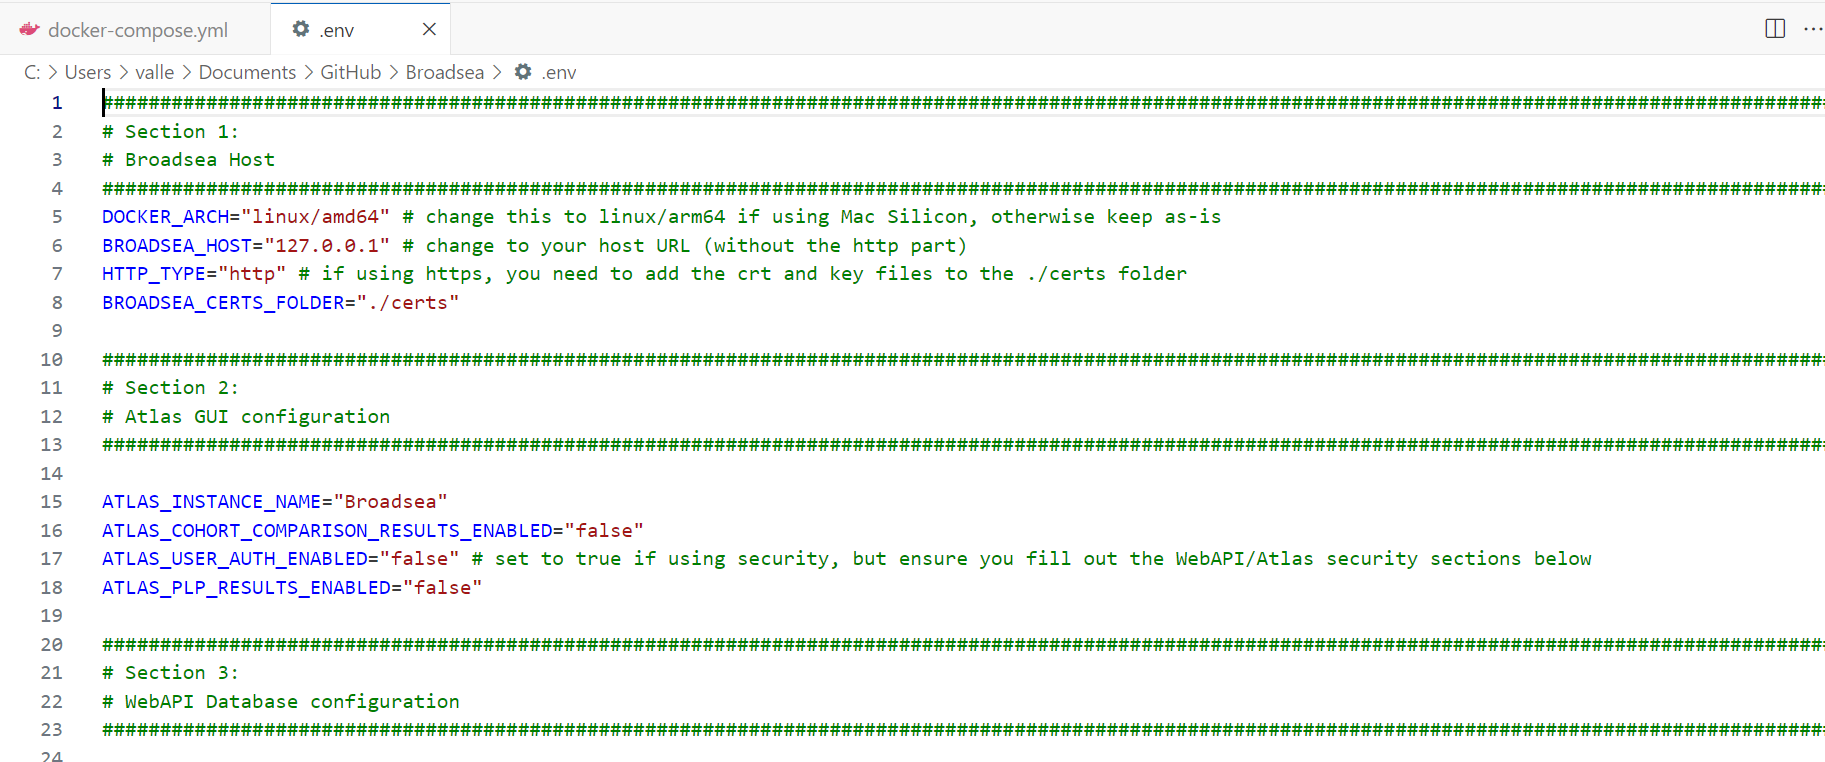
\includegraphics[width=0.90\textwidth]{images/envFile.png}
    \caption{Captura de pantalla del archivo .env del repositorio Broadsea.}
    \label{fig:envFile}
\end{figure}

    \item Por último, para acceder a los servicios de Broadsea hay que abrir en nuestro navegador web (Chrome recomendado) el servidor en el que se alojan los servicios. Por defecto, Broadsea viene configurado para alojarse en el localhost (ya sea en el puerto 0.0.0.0 o 127.0.0.1). Podemos comprobar el puerto exacto revisando la configuración según las intrucciones del punto anterior.

    En este caso, el servidor de Broadsea se aloja en la dirección 127.0.0.1, tal y como se muestra en la Figura \ref{fig:broadseaCap}. Es interesante notar que Broadsea permite el acceso interactivo a la herramienta Atlas, que es la que nos interesa en este caso, pero también a Ares y a Hades, otras dos herramientas muy relacionadas.

\begin{figure}[H]
    \centering
    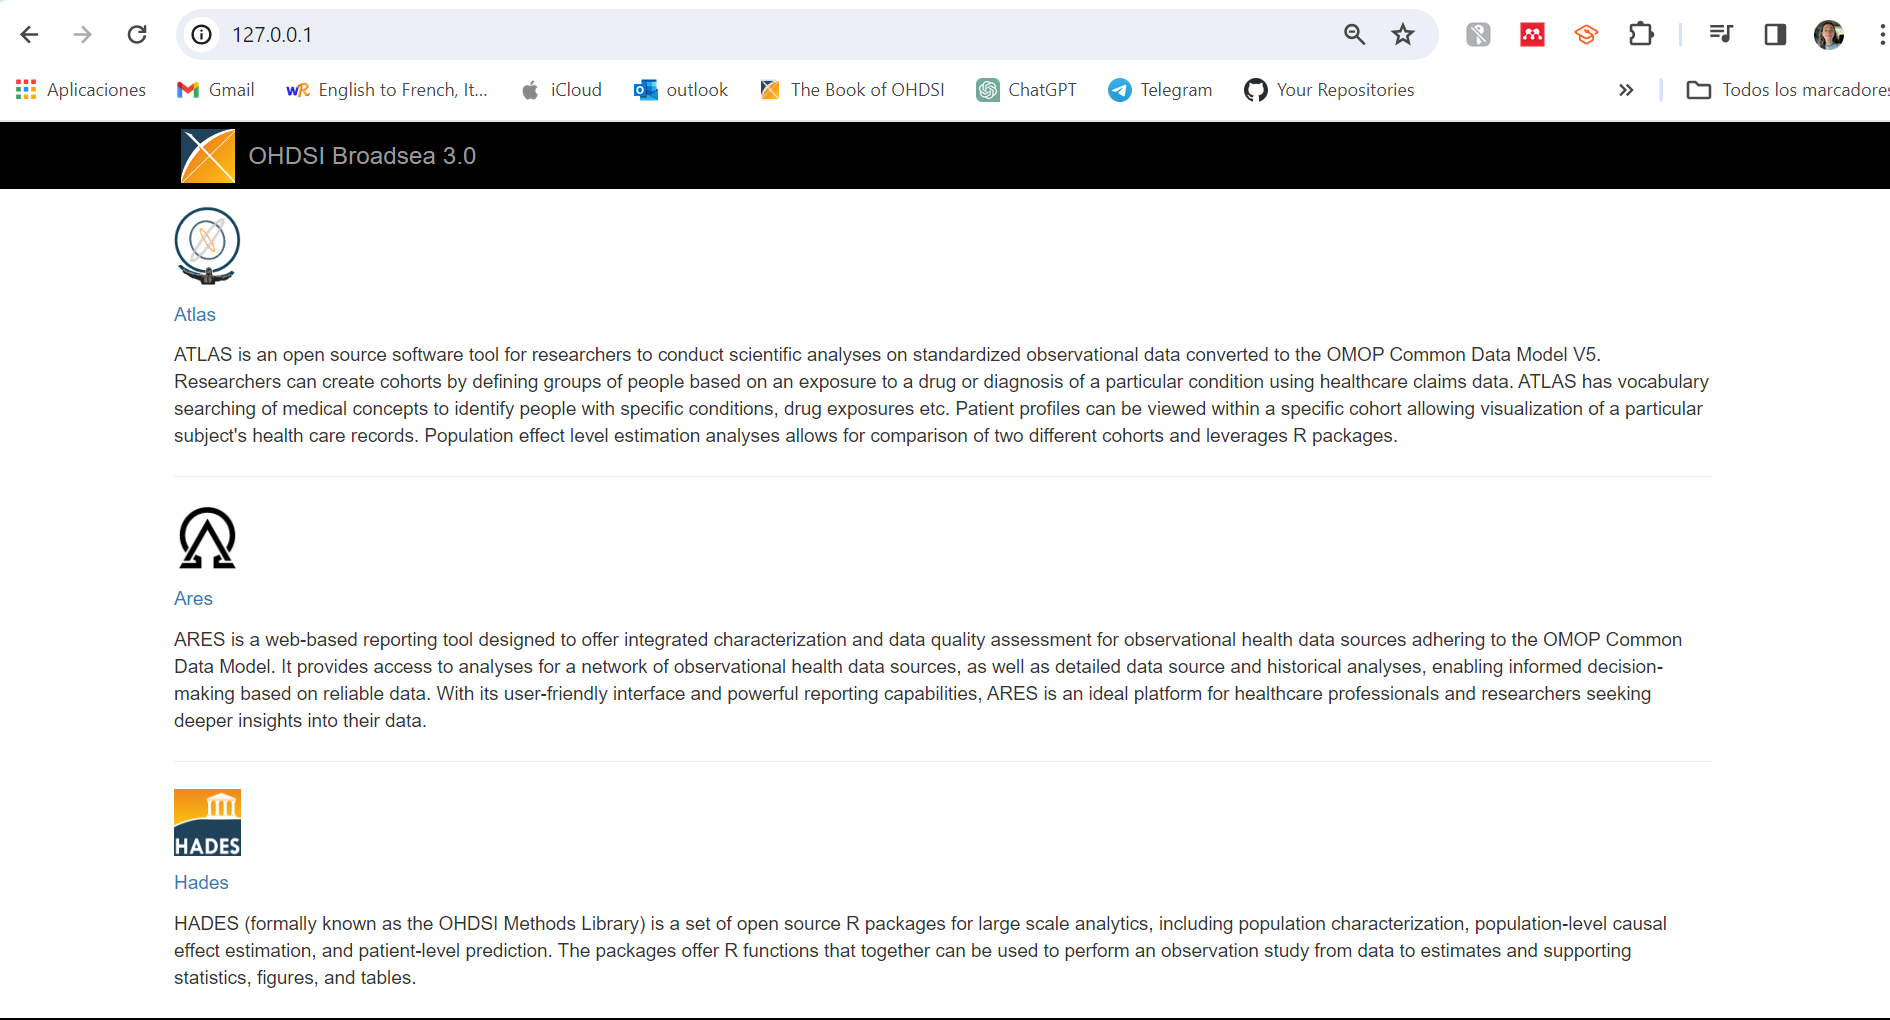
\includegraphics[width=0.90\textwidth]{images/broadseaCap.png}
     \caption{Captura de pantalla del servidor Broadsea ejecutado en Chrome}
    \label{fig:broadseaCap}
\end{figure}

    La ejecución de ATLAS en Broadsea es similar a ATLAS demo, aunque con algunas diferencias. En primer lugar, Broadsea solo ejecuta, por defecto, una base de datos, que es la base de datos de Eunomia.

\begin{figure}[H]
    \centering
    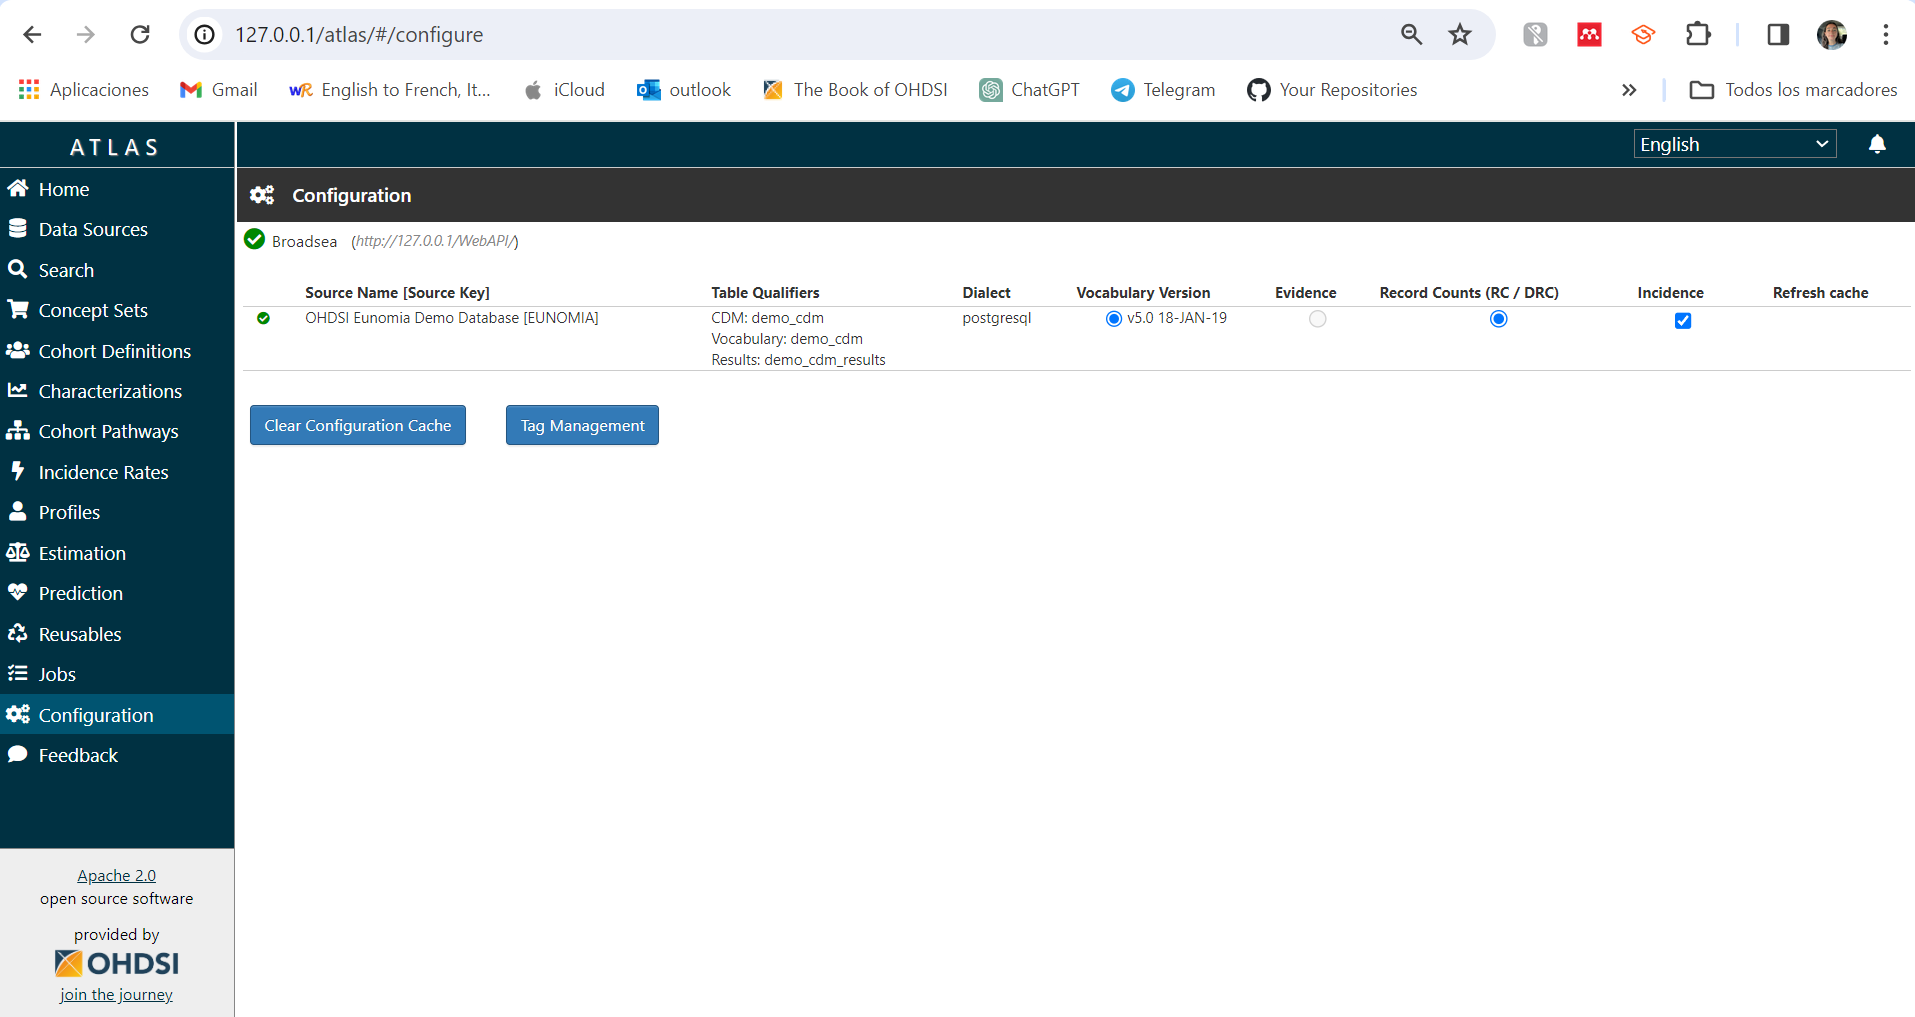
\includegraphics[width=0.90\textwidth]{images/atlasBroadseaDB.png}
     \caption{Captura de pantalla de base de datos que utiliza ATLAS Broadsea}
    \label{fig:atlasBroadseaDB}
\end{figure}

    Por otra parte, y en contraste con la versión demo, ya no aparecen las entradas y estructuras que generan otros usuarios. La herramienta se presenta vacía, para ser completada solo con la información que nosotros introduzcamos.

\begin{figure}[H]
    \centering
    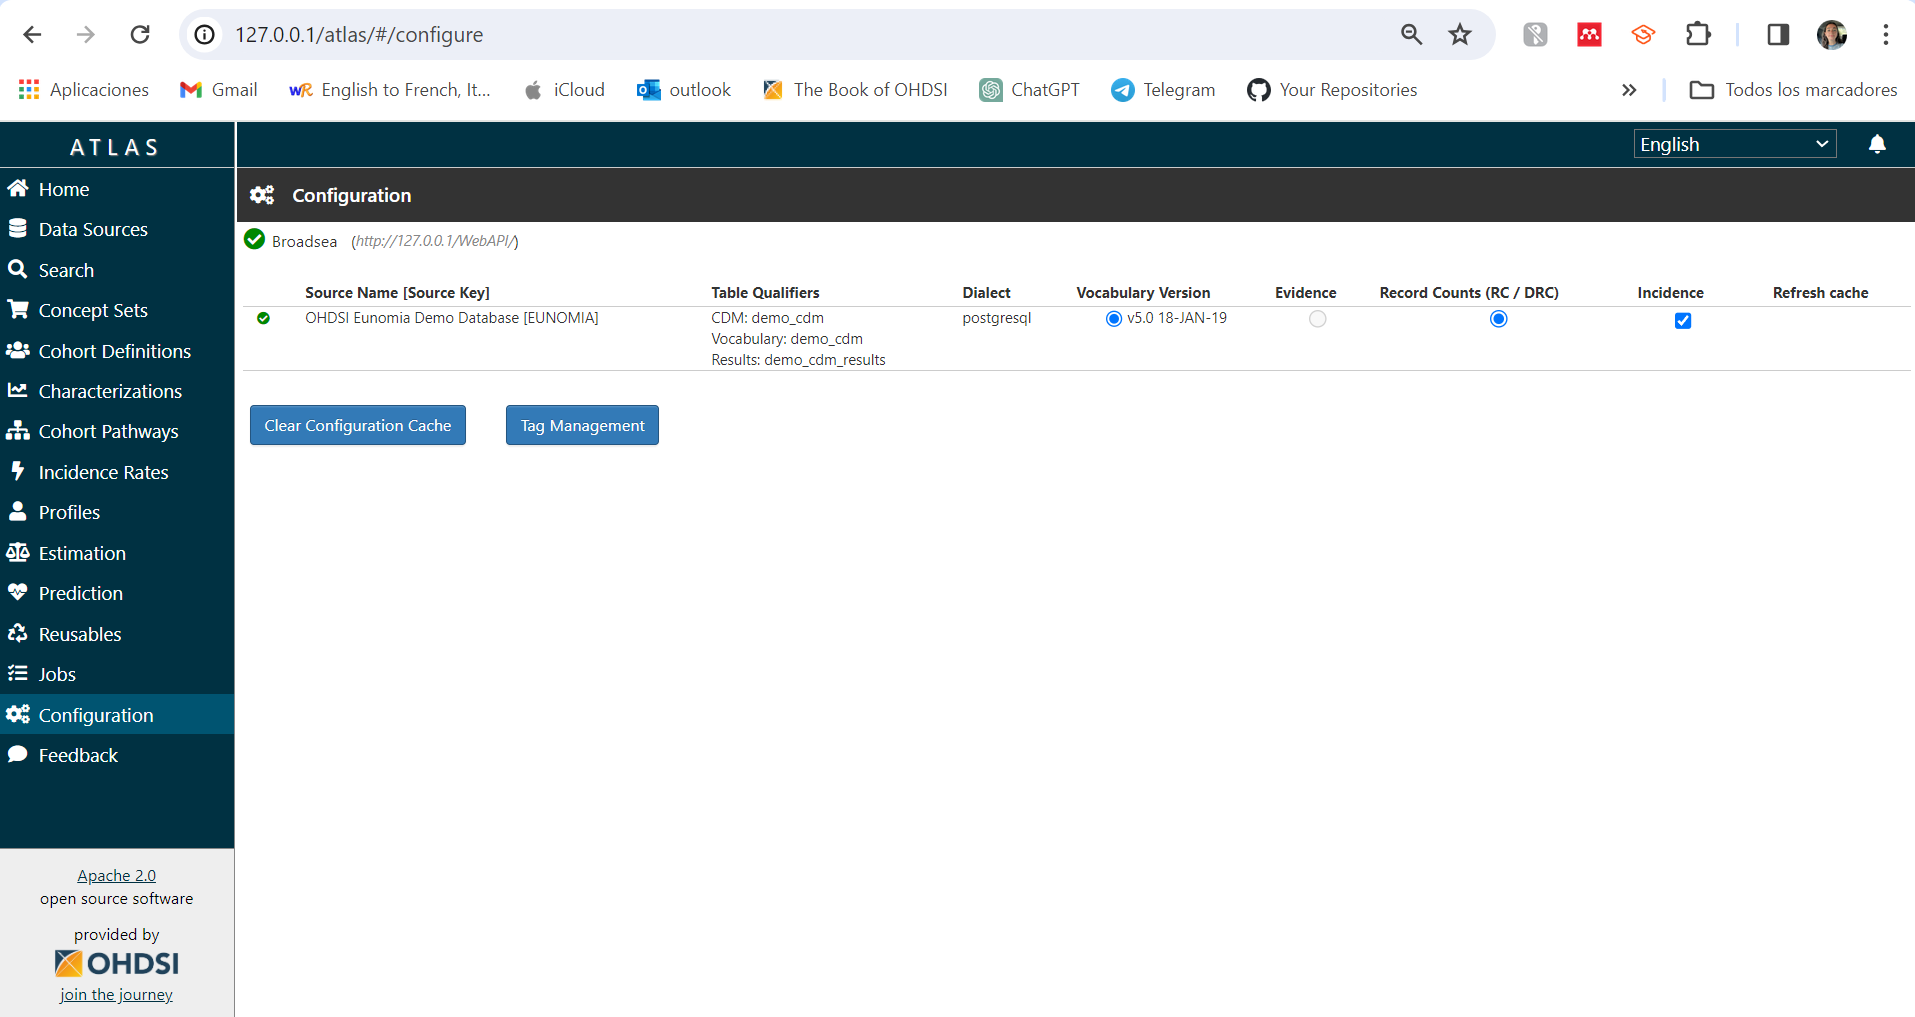
\includegraphics[width=0.90\textwidth]{images/atlasBroadseaDB.png}
     \caption{Captura de pantalla señalando el número de entradas de definición de cohorte que almacena ATLAS Broadsea}
    \label{fig:atlasBroadseaDB}
\end{figure}
    
\end{enumerate}

\textbf{Solución de posibles errores}

%--------------------------------------------------------------
\subsection{Conexión local con la base de datos de Broadsea}

En ocasiones, puede resultar interesante acceder a la base de datos remota de Broadsea desde un administrador de bases de datos local.  Docker almacena las bases de datos que utilizan los contenedores en lo que se denominan \textit{''volúmenes''}. Para revisar los volúmenes que están ejecutándose en el equipo se presentan dos estrategias:

\begin{enumerate}

    \item La forma más sencilla de interactuar con los volúmenes es a través de Docker Desktop, en la sección \textit{''volumes''}. En esta sección se muestran todos los volúmenes que está utilizando el equipo. En este caso, deben aparecer tres volúmenes, entre ellos atlasdb-postgres-data es el volumen de interés, en el que se almacena la información de la base de datos de ATLAS.

\begin{figure}[H]
    \centering
    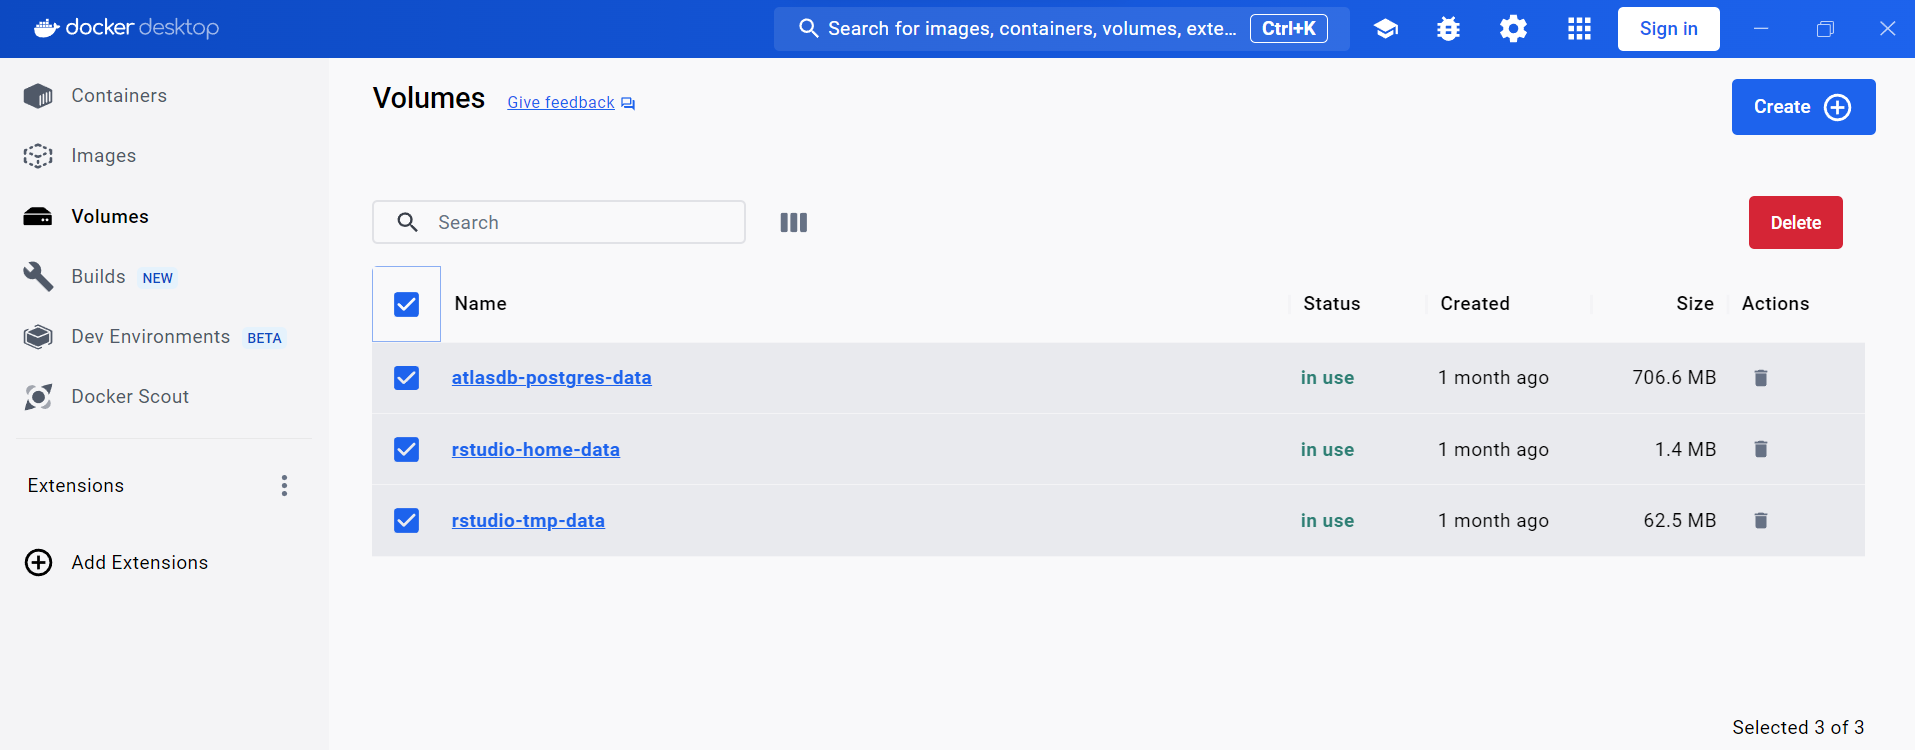
\includegraphics[width=0.90\textwidth]{images/dockerVolumes.png}
     \caption{Captura de pantalla del panel ''volumes'' de Docker Desktop}
    \label{fig:dockerVolumes}
\end{figure}

    \item Otra forma de comprobar el estado de los volúmenes es a través de la terminal del sistema, ejecutando el comando \textit{''docker volumes ls''}, que devuelve un listado de los volúmenes que se están ejecutando.
    
\begin{figure}[H]
    \centering
    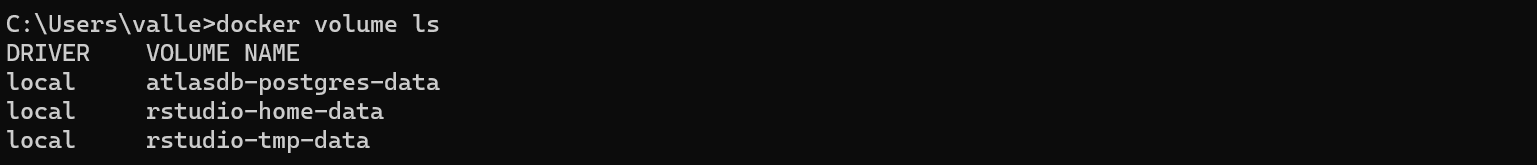
\includegraphics[width=0.90\textwidth]{images/dockerVolumesCDM.png}
     \caption{Captura de pantalla del comando ''docker volume ls'' en la terminal}
    \label{fig:dockerVolumesCDM}
\end{figure}
    
\end{enumerate}

Puede ser importante conocer la información de los volúmenes que ejecuta Docker para identificar comportamientos inusuales y acceder a configuración e información avanzada sobre el virtualizador. 

Por otro lado, la información específica sobre la configuración de los contenedores que utiliza Docker para conformar Broadsea se encuentra en el archivo \textit{''docker-compose.yml''}, alojado en la carpeta local del repositorio de github de Broadsea. Buscando el nombre del contenedor que alberga la base de datos de ATLAS se puede acceder a toda la información relevante del mismo, tal como se muestra en la Figura \ref{fig:dockerComposeDB}. Esta información será necesaria posteriormente para realizar la conexión con la base de datos.

\begin{figure}[H]
    \centering
    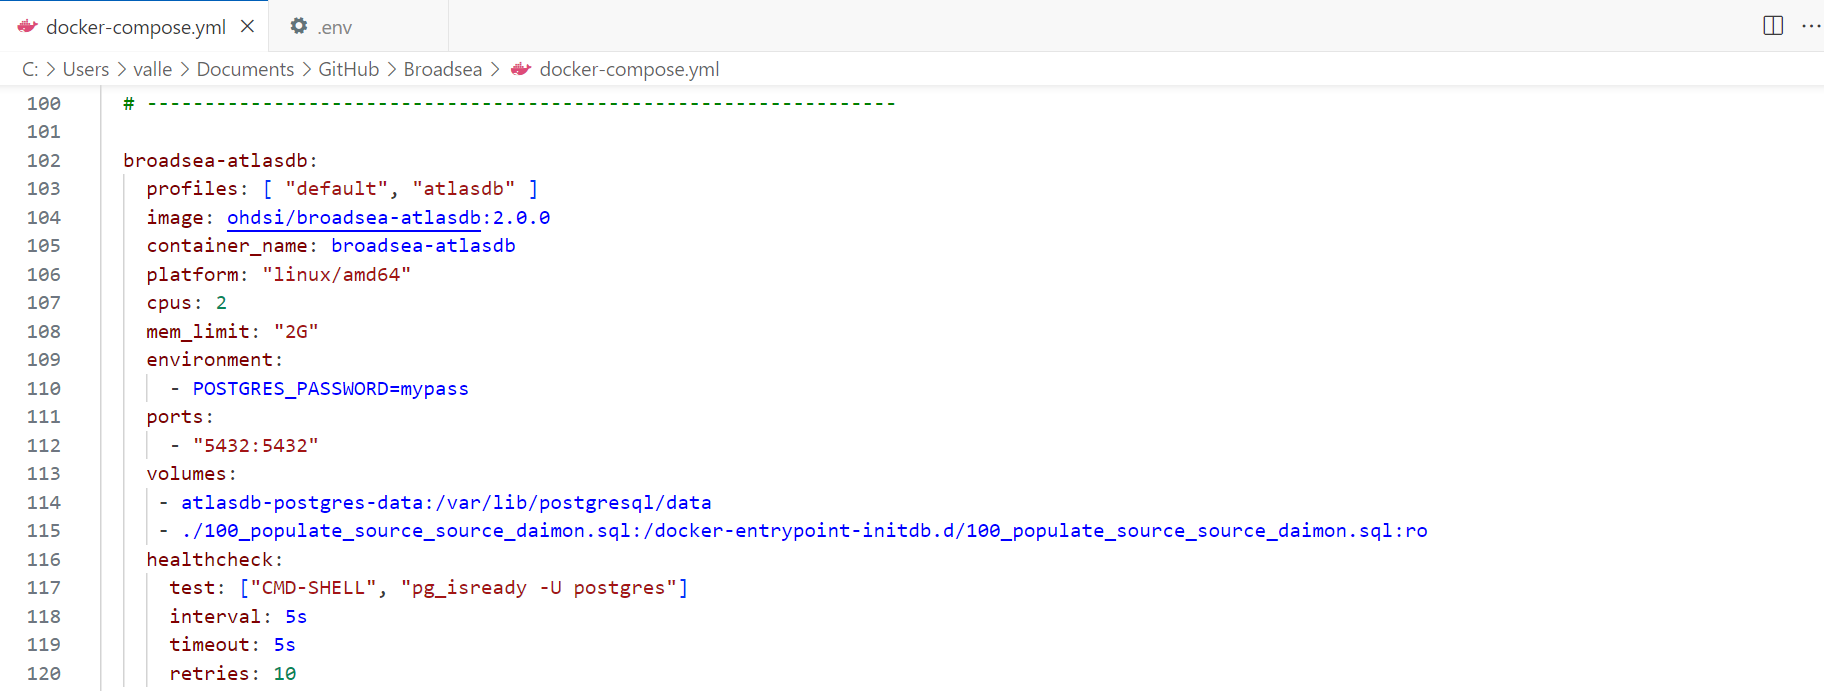
\includegraphics[width=0.90\textwidth]{images/dockerComposeDB.png}
     \caption{Captura de pantalla de la configuración del archivo \textit{docker-compose.yml}}
    \label{fig:dockerComposeDB}
\end{figure}

\textbf{Requisitos para establecer la conexión}

\begin{enumerate}

    \item Descargar e instalar la base de datos PostgreSQL. Lo más sencillo es seguir las instrucciones de la \href{https://www.postgresql.org/download/}{página web oficial} para la descarga y seguir la configuración por defecto para la instalación.

    \item Descargar e instalar una administrador de base de datos PostgreSQL. Se recomienda utilizar el administrador pgAdmin. Para ello, lo más sencillo es seguir las instrucciones de la \href{https://www.pgadmin.org/download/}{página web oficial} para la descarga y seguir la configuración por defecto para la instalación.
    
\end{enumerate}


\textbf{Deployment}

Para establecer la conexión con la base de datos que utiliza Broadsea, se debe seguir las siguientes instrucciones:

\begin{enumerate}

    \item En primer lugar, se debe comprobar los parámetros de configuración de la base de datos. Para ello, se han detallado varias estrategias a lo largo del manual, siendo la más recomendada para esta ocasión revisar el \textit{docker-compose.yml} (Figura \ref{fig:dockerComposeDB}). Este archivo alberga la información técnica de los contendores que ejecuta Docker. En este caso, el contenedor que interesa es \textit{''broadsea-atlasdb''}.

    En el archivo por defecto, se presenta la contraseña para acceder a la base de datos \textit{(password=mypass)} y el puerto que utiliza (\textit{port=5432}).

    \item La configuración por defecto de Broadsea se solapa con la configuración local por defecto de PostgreSQL porque ambos alojan sus bases de datos en el servidor local y en el puerto 5432. Por tanto, para evitar este solapamiento se debe detener el servicio local de PostgreSQL, de forma que el puerto quede libre para albergar la base de datos de Broadsea.

    Para detener el servicio local de PostgreSQL lo más sencillo es abrir la aplicación \textit{servicios} buscar el servidor de postgre y deterlo, tal y como se muestra en la Figura \ref{fig:serviciosConfig}. Así nos aseguramos de liberar el puerto para que pueda ser ocupado por la base de datos de Broadsea.

    \begin{figure}[H]
    \centering
    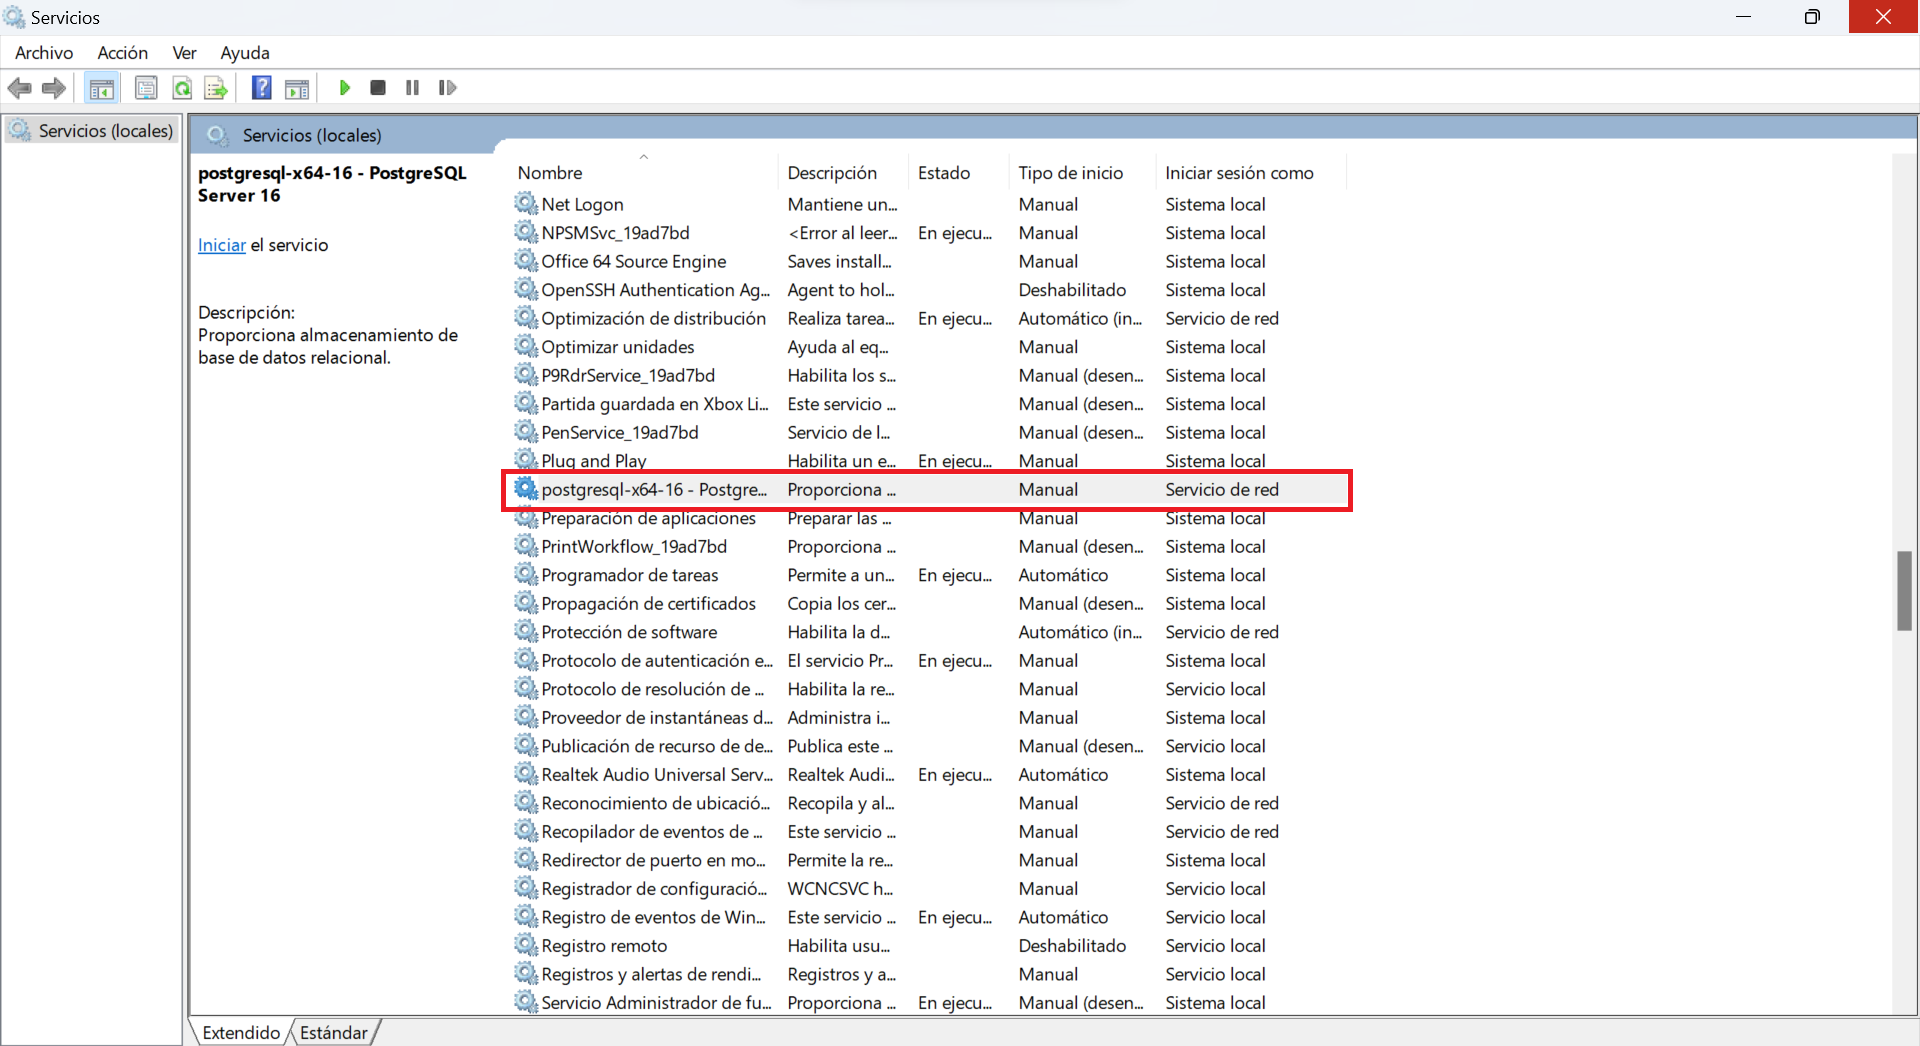
\includegraphics[width=0.90\textwidth]{images/serviciosConfig.png}
     \caption{Captura de pantalla de la aplicación de servicios.}
    \label{fig:serviciosConfig}
    \end{figure}

    \item El último paso consiste en registrar el servidor a través del administrador de base de datos instalado en el equipo, en este caso pgAdmin. 
    
    Una vez que tengamos libre el puerto 5432, podemos registrar un nuevo servidor en dicho puerto que acceda a la base de datos de Broadsea. Para ello abrimos el administrador de la base de datos PostgreSQL, pgAdmin 4, y registramos un nuevo servidor. Los parámetros de configuración de este nuevo servidor se describen en el \textit{docker-compose.yml} y en la sección 3 del archivo \textit{.env}. Los parámetros fundamentales son:

    \begin{lstlisting}[language=sh]
        host = 127.0.0.1
        port = 5432
        user = postgres
        password = mypass
    \end{lstlisting}
    
    \item Tras registrar el servidor correctamente, debe aparecer una base de datos con cinco esquemas: ''demo\_cdm'', ''demo\_cdm\_results'', ''public'', ''webapi'', ''webapi\_security''. Para comprobar que se ha establecido una conexión correcta con la base de datos, sin pérdida de información, se puede comprobar el número de filas que recupera pgAdmin de la tabla ''person'' del esquema ''demo\_cdm'', tal y como se muestra en la Figura \ref{fig:pgAdmin}.

    \begin{figure}[H]
    \centering
    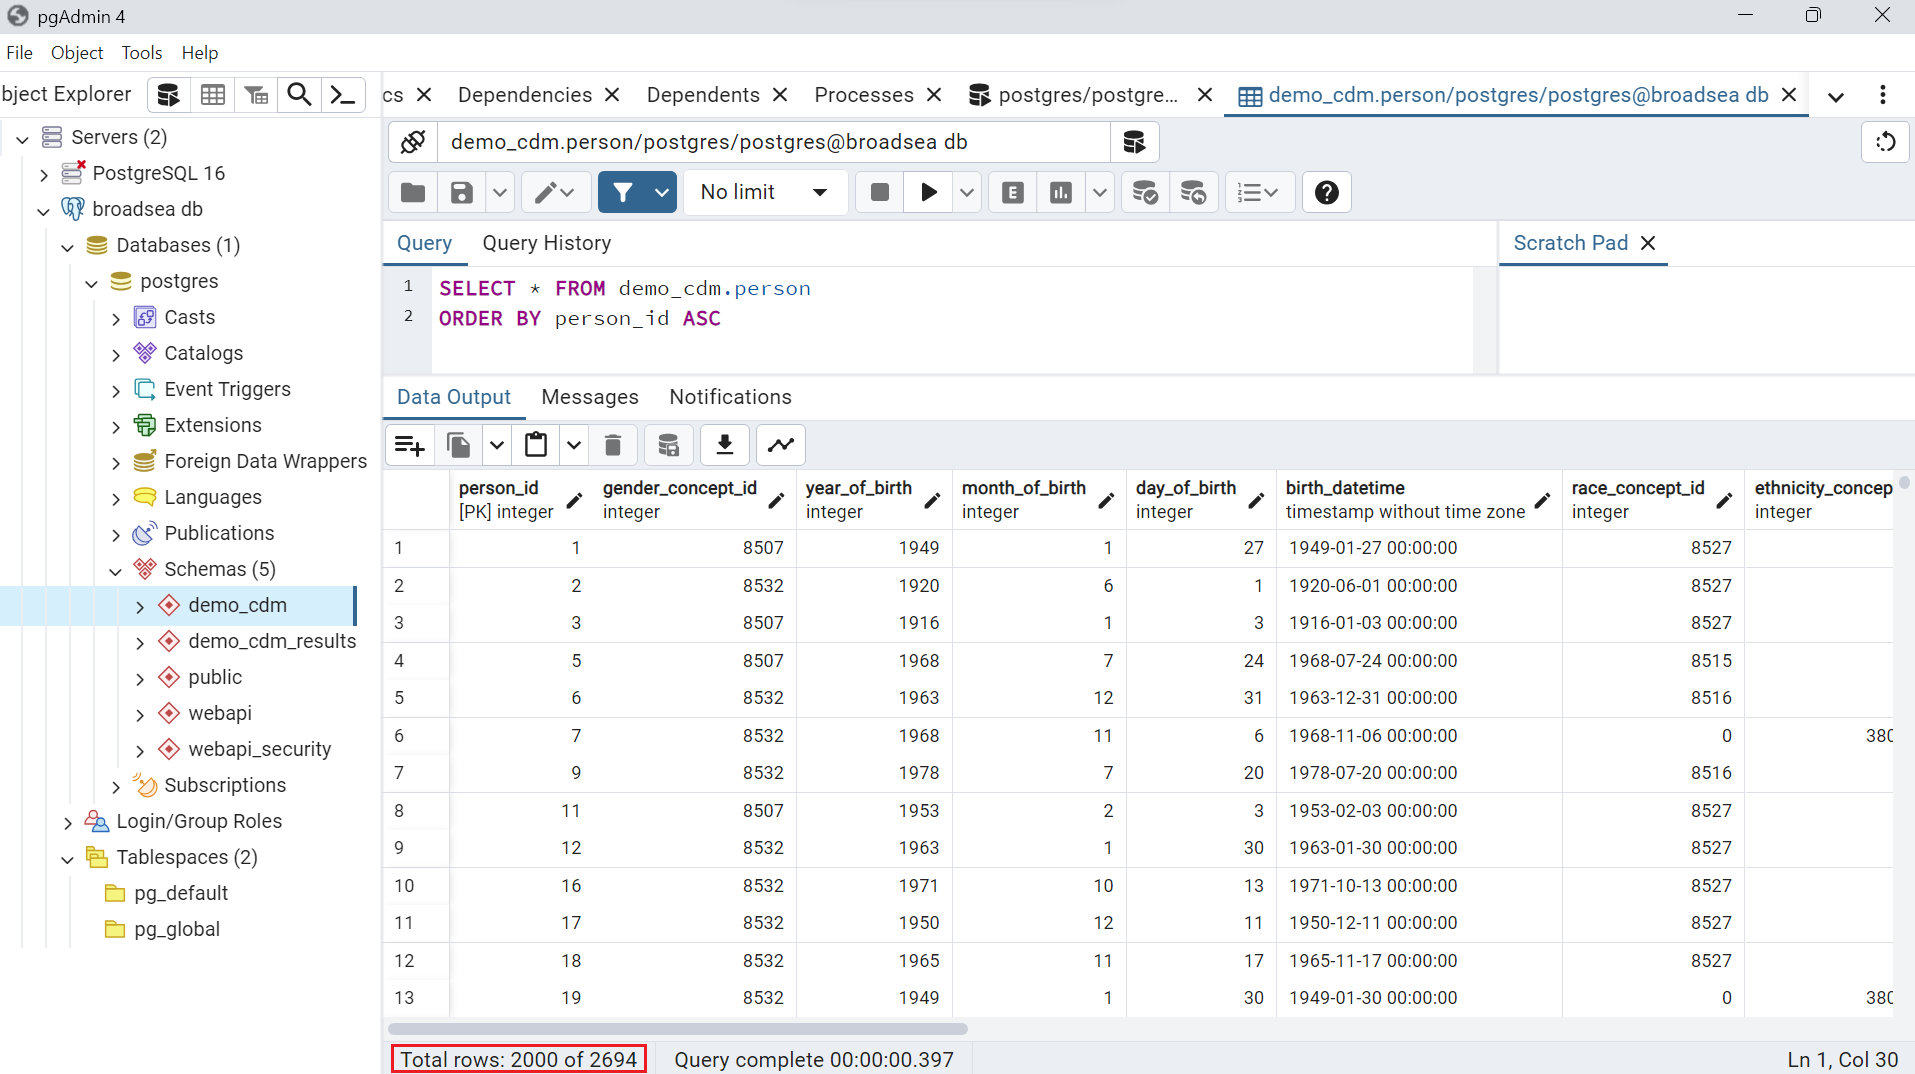
\includegraphics[width=0.90\textwidth]{images/pgAdmin.png}
     \caption{Captura de pantalla de pgAdmin.}
    \label{fig:pgAdmin}
    \end{figure}

    El número de filas que recupere pgAdmin debe ser igual al número de personas que muestra ATLAS en la sección Data Sorce/Dashboard, en este caso son 2694 personas (Figura \ref{fig:DashboardEJ}

    \begin{figure}[H]
    \centering
    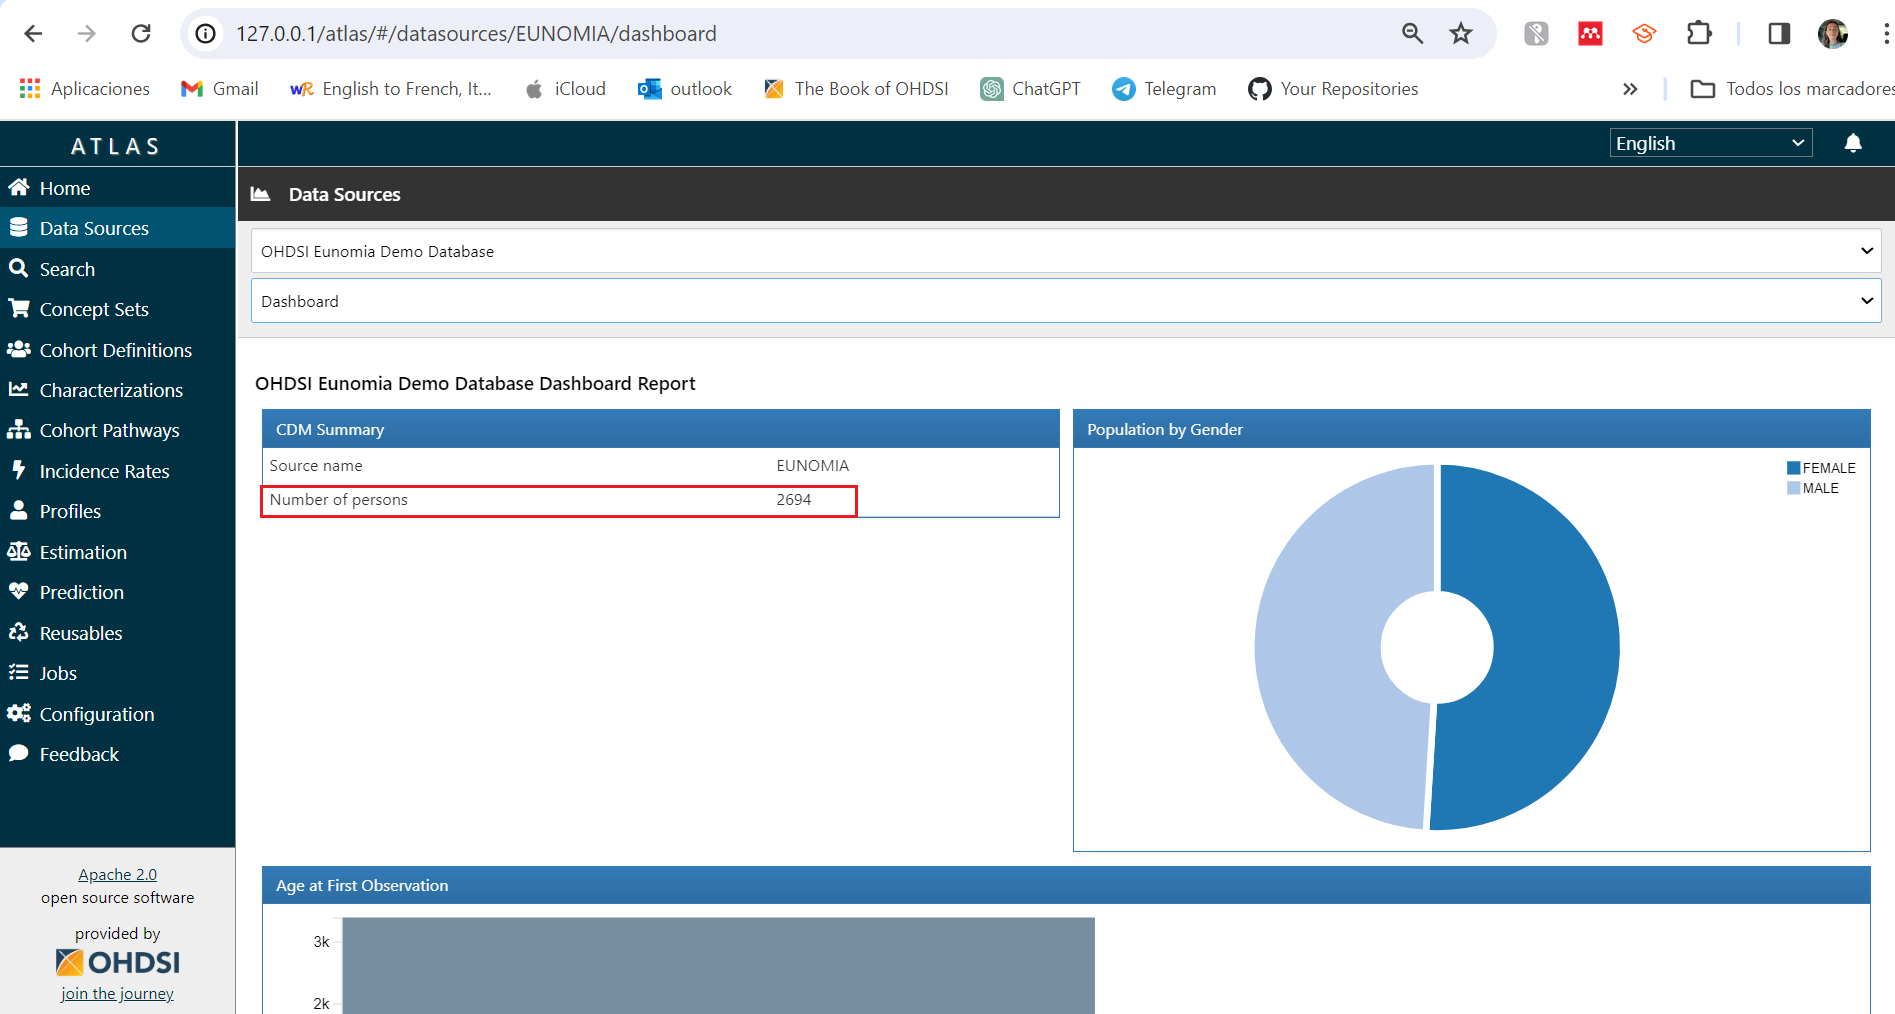
\includegraphics[width=0.90\textwidth]{images/dashboardEJ.png}
     \caption{Captura de pantalla de ATLAS Data Sources/Dashboard.}
    \label{fig:dashboardEJ}
    \end{figure}

    \item Por último, otra forma de comprobar que la conexión es correcta y una forma alternativa de realizarla, con el fin de detectar posibles problemas durante la implementación, es ejecutar el siguiente script de código en R, que realiza la conexión con la base de datos a través de RStudio:

    \begin{figure}[H]
    \centering
    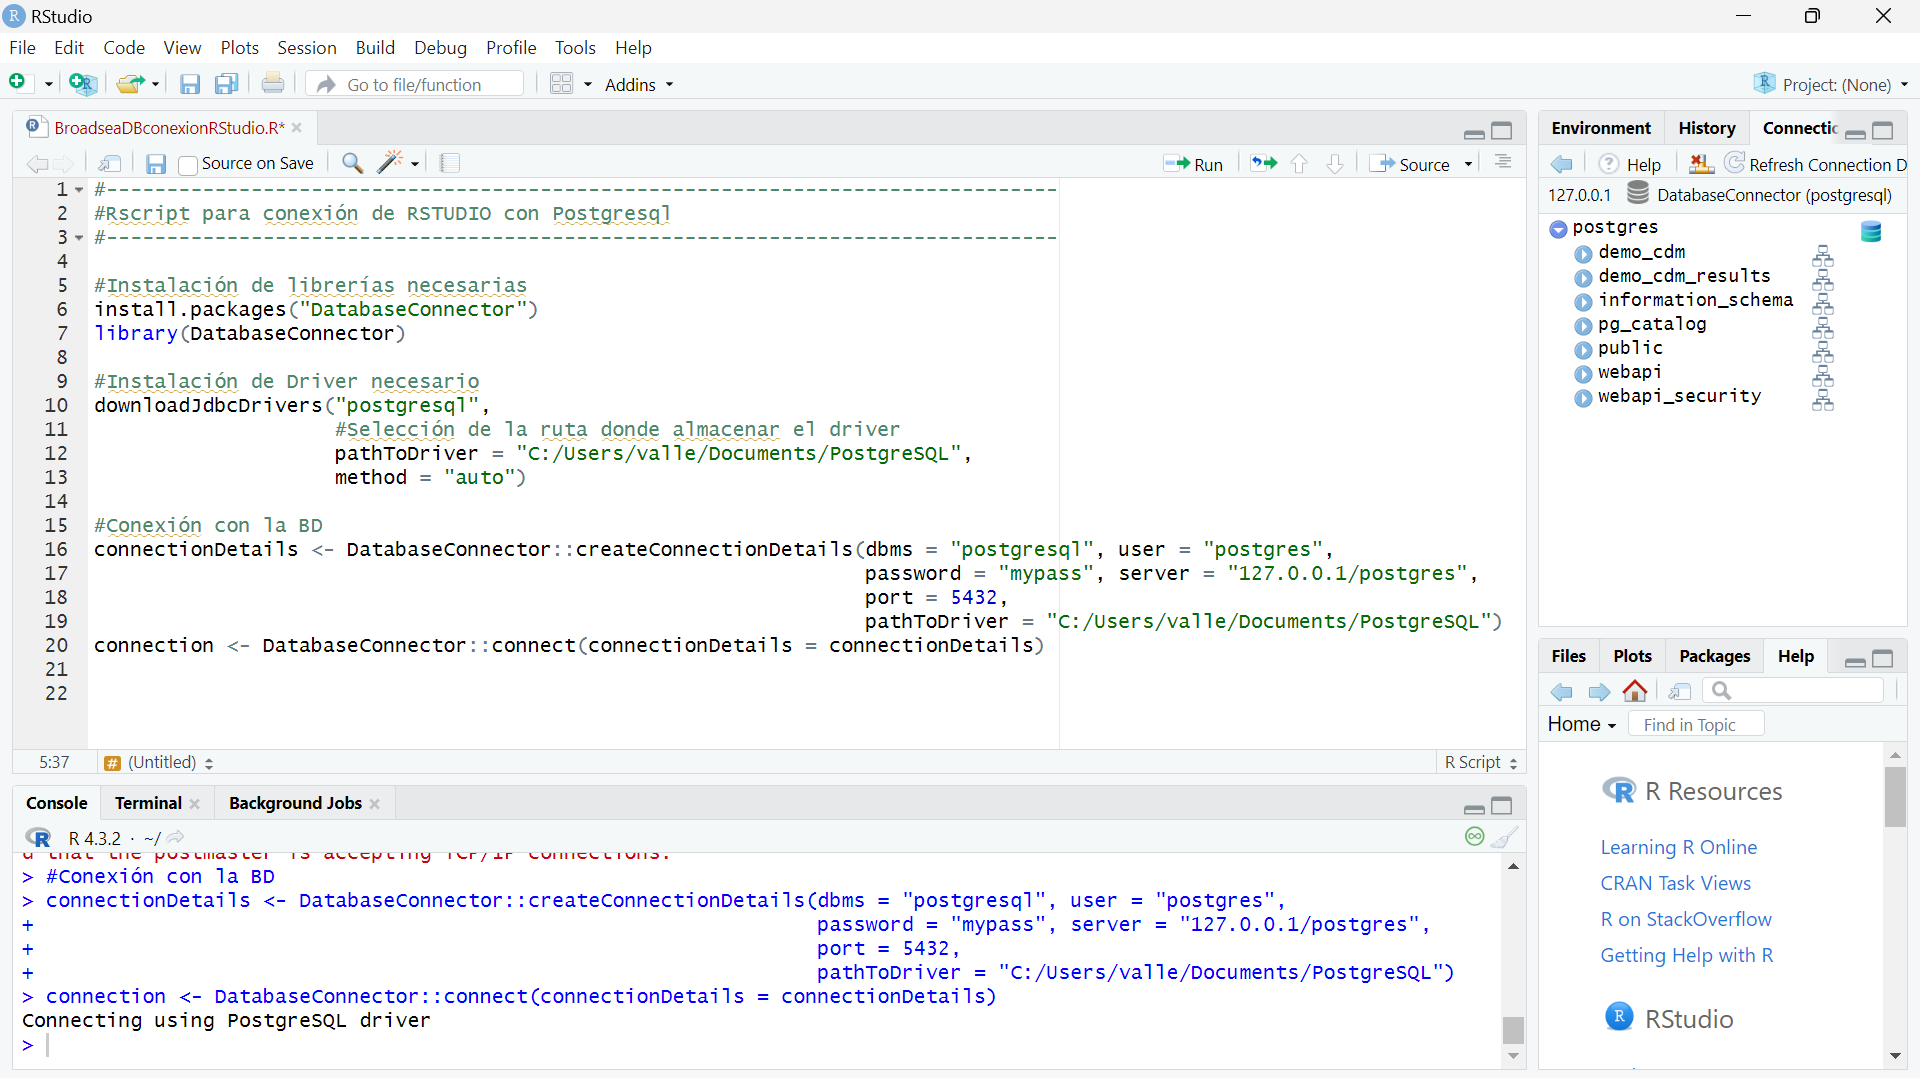
\includegraphics[width=0.90\textwidth]{images/RStudio.png}
     \caption{Captura de pantalla de script de RStudio.}
    \label{fig:RStudio}
    \end{figure}
    
\end{enumerate}

\textbf{Información sobre la bd de Broadsea - Eunomia}

\textbf{Solución de posibles problemas}

- No permite establecer la conexión

- Acceder a postgre sin haber encendido el contenedor
- 

\subsection{Subir base de datos local a Broadsea}


- Mediante SQL queries
- Activando la seguridad









%%------------------------------------------------------------------
%% 2.3 ATLAS AWS
%%-------------------------------------------------------------------

\newpage
\subsection{ATLAS AWS}\label{cap:AtlasAWS}

Otra alternativa para la implementación de herramientas OHDSI como ATLAS en una organización es utilizar Amazon Web Services. La naturaleza gratuita y de código abierto de OHDSI significa que estas capacidades están disponibles para organizaciones de cualquier tamaño. La agilidad, escalabilidad y bajo costo de la infraestructura de AWS permiten el uso extenso y consistente de OHDSI sin una inversión de capital significativa o esfuerzos prolongados de TI. La gestión detallada de capacidad de Amazon Redshift Serverless y Amazon Aurora Serverless permite ejecutar cargas de trabajo de investigación variables e impredecibles a bajo costo \cite{OHDSIAWS}. 

Por tanto, aunque el costo es bajo, es importante saber que esta alternativa no es gratuita.


\textcolor{red}{https://github.com/OHDSI/OHDSIonAWS?tab=readme-ov-file}

\textcolor{red}{- OHDSI-in-a-box versión AWS}

\textcolor{red}{- OHDSIonAWS}

%%------------------------------------------------------------------
%% 2.4 ATLAS local
%%-------------------------------------------------------------------

\subsection{ATLAS local} \label{cap:ATLASlocal}

La instalación local de ATLAS es la más compleja de todas porque requiere instalar todo el entorno de variable y configuraciones del sistema en el ordenador personal de forma manual. No obstante todo este proceso está correctamente documentado en las wikis de github \cite{AtlasSetup} y en el curso de EHDEN Academy \cite{EHDENAcademy} ''Infraestructure''. Para realizar la instalación de ATLAS localmente debemos seguir los siguientes pasos:

\begin{enumerate}
    \item Instalación de la WebAPI
    \item Instalación de ACHILLES
    \item Instalación de NodeJS
\end{enumerate}


%%------------------------------------------------------
%% 3. FUNCIONAMIENTO
%%------------------------------------------------------

\newpage
\section{Funcionamiento de la herramienta.}




%%%%%%%%%%%%%%%%%%%%%%%%%%%%%%%%%%%%%%%%%%%%%5
\newpage
\bibliographystyle{plainnat}
\bibliography{sample}

\end{document}